\chapter{Context of the Work}

\label{Chapter1}

\section{Introduction}
The work is based on an Industry 4.0 scenario, which is a cyber-physical environment consisting of various different 
actors and objects involved. The different actors involved are either stationary or mobile. Moreover, complexity of the 
environment increases when we account for heterogeneous actors with various decision making capabilities. Robots with various
manufacturers present various transform frames, different software and sensors. Due to the heterogeneous nature of the robots 
involved, we can not depend on information we receive from the robot, as this particular information will differ from a robot 
to other based upon it's configuration. The problem is solved by creating a digital twin which records the information of the 
environment as well as the robot. The simulator is dedicated to capture the digital twin of the robot, whereas a script
saves the log values of the obstacle space in a semi-structured format to be used later.

\subsection{Structure of the Report}
The report is structured in four chapters. The first chapter provides context to the work and introduces concepts required to study and 
implement the work. The second chapter details the technologies involved in the project, hardware and software. In the third chapter, 
details about implementation of technologies learnt from chapter two is discussed. The solution to problem is discussed in the fourth chapter 
and the report ends with a conclusion detailing the perspective of the work. 

\section{Motivation}
The structure of a dynamic Industry 4.0 environment is highly volatile, the structure is defined through a stationary frame that 
has been declared before. The decision making capabilities of the robot to navigate the environment while avoiding obstacles and 
other robots can have a great impact on the performance and the utility of the environment. 

\section{Robot}
\subsection{What is a Robot?}
The origin of the word robot can be found in Czech playwriter Karel Chapek's play titled "Rossum's
Universal Robots (R.U.R)" in 1921. Thw word robot results from combining the Czech words \textit{rabota} meaning 
compulsory work and \textit{robotnik} meaning an agricultural bound labor. A \textbf{robot} is a system existing 
in a physical world, with decision making capabilities of varying extent, can sense the environment it's in to achieve
some goals. A goal can be differ according to the need of autonomous behaviour. Essentially, robot is a cyber-physical system 
combining sensing, actuation, and computation. With the advancements in technology and materials essential to build a robot, we can
see numerous different robots with different applications. Robots such as : 
\begin{itemize}
    \item a self-foldable / self-actuated robot developed at MIT \cite{Sung2016ComputationalDO}
    \item a lightweight aerial robot developed at University of Penn
    \item consumer-grade drones by DJI 
    \item Autonomous Vehicles developed at Google.
    \item Autonomous Surface Vehicles by ASV Global
\end{itemize}
Robots help humans to do \textit{dirty}, \textit{dull}, or \textit{dangerous} tasks that no human wishes to do, although they are
important to be done. As any machines, in an Industry 4.0 environment humans can integrate robots into the development/production process,
thus these processes can be optimized. Optimizing robots with different applications can help us to exploit robot technologies to leviate pressure
imposed by growing population by using in applications such as, \begin{itemize}
    \item  mobility-on-demand
    \item  automated highways
    \item  drone swams for servillance
    \item  truck platoons for long distance logistics
\end{itemize} Along with these mobile wheel bearing vehicular robots, we have other robots as : 
\begin{itemize}
    \item autonomous behaviour on any terrain for search and rescue with Big Dog robots.
    \item Persobal Robots for help with menial tasks, for example, iCub Robot.
    \item Emotional Robots wit Human Computer Interface designed to ease the interaction for example, Pepper Robot.
\end{itemize}

\section{Autonomous Behavior}
For a robot to perform autonomous behavior in an environment, it must be able to model and percieve the world it is in, be able to process information
and perform required actions and plan it's behavior in adverse conditions. The level of such autonomy varies with different use cases. These challenges
are solved by deploying perception module, action module and decision-making module. These three modules will be mounted and developed on a cyber-physical
system, differentiate cyber-physical systems with pure artificial intelligence. Architectures employed in Robotics combine the three modules
to be used by the developer to develop such CPS systems.
\subsection{Perception}
For a robot to initiate any form important autonomous behavior of decision making, the robot should know where the robot is present in the given Industry 4.0 environment. A robot uses different sensors to infer it's position in the environment. A
sensor is an entity that is used to measure the state of the world as well as the state of the robot relative to the world. 
The different sensors provide measurements of the environment and extract meaningful information for autonomous behavior. \textbf{Proprioceptive sensor} in a robot is used to determine the coordiante location of the robot relative
to the frame it is in, by measuring internal information to the robot. Proprioceptive sensors can also measure odometry, speedometer, energy level and acceleration of the robot. These coordinates on change define the movement of the robot. Another exteroceptive sensor is used to acquire information regarding the environment the
robot is currently present in by calculating light intensity and sound amplitude to measure the distance from theh nearest obstacle. The perception module will save the information about the map to be
inherited in other modules. \textbf{Exteroceptive Sensors} measure something external to the robot, i.e the environment. Exteroceptive sensors are of two types : 
\begin{itemize}
    \item \textit{Active} : These sensors affect the environment by emitting energy. Examples would be, calculating distance with Infrared Sensor, sonar range finder and calculating distance with laser scanners.
    \item \textit{Passive} : These sensors have no affect on the environment, for example, the ambient light sensor, a sound sensor or camera being used to sense vision.
\end{itemize} 

\subsection{Action}
Action module decides the force and orientation for a robot to perform the task assigned. Action module deals with low level control of the robot's motor. In presence of a predefined goal, 
the action module will calculate the rotational and forward velocities to reach the goal. Action module comprises of various equations responsible to calculate the linear and angular velocities.
\subsection{Decision Making}
In order to achieve a higher order goal, the robot will use the action and perception modules to initiate \textit{navigation} to reach a predefined goal. 
\textbf{Perception} module has provided the neccesary information to the robot about the environment and location of obstacles. \textbf{Action} module provides 
the neccesary equations to calculate the velocities to pursue the motion towards the goal. Delibrative planning is executed by the decision-making module to compute a 
path that does not collide with the obstacles and respects robot's motion constraints. In real Industry 4.0 environment, we've multiple robots and mobile entities. Collaboration, communication
and coordination among the robots for path planning to calculate efficient algorithms for calculating linear and angular velocities are an interesting subject for research.
For example, collective movement between robots as well as aerial unmanned vehicles such as drones can be initiated by either having a distributed architecture or a centralized leader-follower control.
A decentralized system is prone to failure much more than a leader-follower control system. A decision-making algorithm could be written in the leader-follower control system to be in a certain range
or perform a certain action around the leader robot. Multi Robot control and coordination allows us to recreate this. 

The simplest example of an autonomous robot would be the Roomba robot, which is employed to clean our houses. The robot would use the sensors to infer the world i.e the room around him and 
initiate navigation to the most suitable location. A simple roomba robot had, 1) A cliff sensor to make sure the robot is not falling off a level field. 2) A bump sensor to retrack it's behaviour and initiate recovery motion. 3) A wall sensor to detect the walls and distance to it. 4) An optical sensor to detect the odometry and force being exerted by the motor.
The behaviour displayed by the simple robot is :  
\begin{itemize}
    \item \textbf{Wall-Following}: The robot would follow the wall if it bumps into something.
    \item \textbf{Straight} : The robot would go straight and turn a random angle if it bumps into something.
    \item \textbf{Dirty Spot} : If the robot is in contact with a dirty spot, it will spiral around the position untill it bumps into something.
\end{itemize}

This behaviour is very naive and primitive in relation to what robots can do in current scenario and advancements in the last two decades are huge.

\subsection{History}
The field of robotics emerged from combining and taking influences from various different fields which were present at a time around 1950s.
Robotics can see it's influences from : 
\begin{itemize}
    \item \textbf{Control Theory} : Control theory \cite{enwiki:1039308545} develops methods for control of dynamic systems and engineered processes in an environment. The objective is to build a model or an algorithm to decide the behaviour of the entity once a particular trigger event (or an action request) has been initiated, the decided behaviour will influence the state transition to drive it into a desired state while minimizing any delay, overshoot, steady-state behavior while ensuring stability often to achieve a degree of optimality. A controller is present in the robot to decide this behaviour. In robotics, the most important part of controk theory is to control the feedback.
    \item \textbf{Cybernetics} : Cybernetics \cite{enwiki:1037814219} is an interdisciplinary approach important to regulate the structure and control of a device. The outcomes of the actions are further fed into the feedback loop. It is the integration of sensing, action and environment. 
    \item \textbf{Artificial Intelligence} : In 1950s, artificial intelligence dealt with planning processes and reasoning which integrated to develop into robotics.
\end{itemize}
Robotics shifted in 1980s, with introduction of new ideas such as 1) reactive control 2) hybrid control and 3) behaviour based control which produced faster and intelligent machines. Artificial Intelligence's approach to solve a robotics problem shifted from initiating
a delibrative planning algorithm such as shortest distance. Instead robotics tried to imitate living objects and focussed on what an intelligent machine would behave like. By taking inspiration from organisms in nature, it was found that they follow a simple pattern of reactive rules to an external stimuli. This gave rise to reactive behaviours being applied into robotics.
Behaviour based robotics was a key concept for the development of robotics at that point of time.  We could use this behaviour based robotics concept and employ it in concepts such as swarm robotics and collective intelligence, thus birthing a new research area in robotics itself.
As years passed, and we had improvements in computation and hardware design for the sensors, we moved away from the behaviour based robotics. We still see concepts such as wall-following, obstacle avoidance is based upon behaviour based control paradigm.
A huge trend recently is in leveraging neural networks and machine learning to improve the perception and control of the robot. Researchers are trying to integrate machine learning end to end in the robot itself promoting it's intelligent behaviour. As we use the robot's as a blackbox, with an end to end architecture it is very difficult for us to understand why a robot is doing what it is doing at a certain position.
In our work, we are trying to record this behaviour of the robot while considering it as a black box with an end to end architecture and learning it's behaviour by making a digital twin.
\section{Robot Control Architectures}
The building block of an autonomous system such as a robot is a perception-action loop. Perception-Action loop is a cycle for the robot to process the thing that he experiences and the things that he does, simultaneously improving the decision making process of the robot. The robot is in a continous interaction with it's environment. 
\begin{itemize}
    \item \textbf{Reactive Control} : Reactive Control deals with using the sensors to present the current estimate of the world, recovery behavior rules in case of collision produce actions which are simple and fast to compute.
    \item \textbf{Delibrative Control} : Delibrative Control deals with predicting the future state of the robot, developing a plan for the same for the robot to decide the \textit{sequence of actions} to pursue in order to follow the sequence. In our work, we have used delibrative planning to move the robot from a starting position to the goal position via different algorithms ; for example A\textsuperscript{*}, Dijkstra and Greedy Best First Search Algorithm is used to compute the path of the robot.
\end{itemize}
Complicated actions require complicated control architectures, which combine the three elemental modules of autonomy which are perception, plan and action. Examples of such control architecture are,
\begin{itemize}
    \item \textbf{Finite State Machines} : They are reactive and follow a sequential path. Consisting of a finite set of states and transitions between these states. A simple example in this case would be 'pick up the trash' robots.
    \item \textbf{Subsumption Architecture} : They are reactive and follow a concurrent path, which means that the three modules of perception action and decision making will execute simultaneously.
    \item \textbf{Sense-Plan-Act} : They follow a delibrative path planning method which use the modules in a step by step way.
\end{itemize}

\begin{figure}[th]
    \centering
    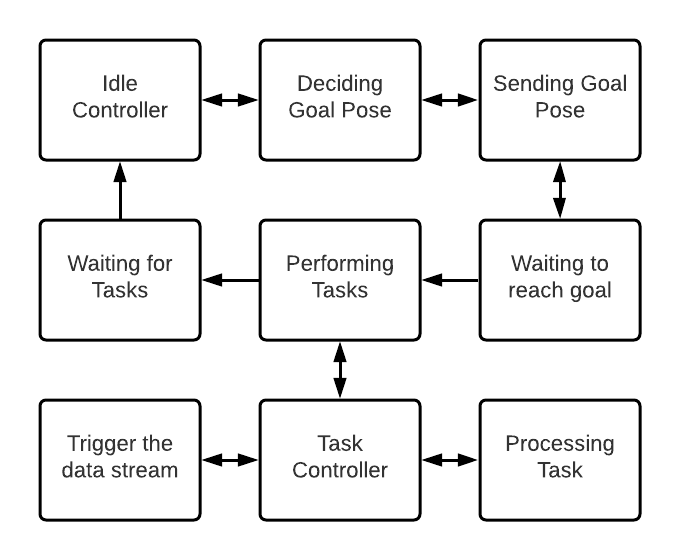
\includegraphics[width=0.6\textwidth]{Figures/controller-process.png}
    \decoRule
    \caption[]{State Diagram of Controller}
    \label{fig:StateDiagController}
\end{figure}

As seen in the Figure~\ref{fig:StateDiagController}, the motor controller is dynamic. The controller carries multiple processes simultaneously for the robot to move autonomously.

\section{Motion Control in Robots}
Motion Control in a robot deals with the process through which the delibrative or reactive control is passed down to actuators of the robot and finally to the motor resulting in the physical change of state in a direction robot's decided to move to. The action component of the autonomy controls the robot with the motion control module.
\subsection{Actuators}
Actuators are used to convert a signal from a circuit board, e.g. from a Raspberry Pi or an Arduino into physical mechanical motion. Actuators serve various purposes, such as locomotion, manipulation, heating and sound emission. 
Other examples of electrical-to-mechanical actuators are, DC Motors, stepper motors and loudspeakers. \textit{For example, } in a normal example of an automated car a driver can steer and acclerate, thus making 2 control points.
There are examples of for uncertainty and noise in actuators. Examples of such are wheel slip, slack in the motion and environmental factors such as wind, friction and other natural uncontrollable distractions. Actuators influence a certain single degree of freedom of the robot.
A robot is controllable in all of it degree of freedom if it has an actuator at each and every degree of freedom. \textit{Degree of Mobility } is the number of DOFs which are operable by the actuators. If the DOF is equal to robot's DOM the robot is a \textit{holonomic robot} and if the number of DOF is greater than it's DOM then it is a \textit{non-holonomic robot}. Otherwise, if robot's DOM is more than it's DOF, the robot's actuation is redundant.
The robot in our project is a \textbf{Differential Drive Robot} which can actuate with left and right wheels without any interference. DDR has 3 DOF but DOM is 2, differential drive robots are \textit{non-holonomic} in nature.  
\subsubsection{Kinematics}
Kinematics are important for us to infer and calculate the motion, i.e behaviour of the robot when it reaches a goal.
Forward Kinematics decide where the robot would end up in the coordinate frame of the environment $(x,y,\theta)$ given that we have the control parameters and the time of movement. Reverse kinematics deal with finding the control parametetrs of the robot once the desired final position $(x,y,\theta)$ is provided.

 \section{Localization}
Localization deals with positioning a robot in the coordinate frame of the environment. When you put a robot randomly in an Industry 4.0 environment, it does not know where it is or how the environment around the robot looks. There are various methods with which one can accomplish localization. 
\textit{Dead-Reckoning}, is an initial/minimal method of localization where we know the initial position of the robot, and we further update the position of the robot blindly based on the differential movements. Thius method is odometry-based. 
\textit{Global Localization}, is a method where initial position of the robot is not known. There are two major methods to infer the position of the robot and initialize localization :
\begin{itemize}
    \item \textbf{Map-Based Localization} : In this method, we have various landmarks or obstacles which we can develop into a map. Sensors employed in this method are, laser sensor, camera for vision and proximity sensors. There are various map-matching techniques used to develop a map.
    \item \textbf{Beacon-Based} : In this methods, we employ an active infrastructure with bluetooth, WiFi, GPS Sensors for outdoors. The method used here is trilateration, fingerprinting and proximity.
\end{itemize}


In our implementation, as well as major implementations across different robotics projects. The project employs a combination of global localization and position tracking methods.
There are multiple challenges faced by localization in dead-reckoning and global localization : 
\begin{itemize}
    \item \textbf{Dead-Reckoning} \begin{itemize} \item a slip could occour in the wheel, thus displacing the localization and producing an error \item errors caused by runaway \end{itemize}
    \item \textbf{Global Localization} \begin{itemize} \item various errors and failures \item noise in the non-Gaussian sensor \item unreliability of sensors access such as GPS \item ambiguous map \item environments which are continuously changing with dynamic obstacles \item a robot is not able to know that it has been displaced, so it still displays the position relative to the previous reference frame.  \end{itemize}
\end{itemize}
\subsection{Probabilistic Localization}
In robotics, we employ localization probabilistically. The three key components to such localization are robot's information related to where it is (it's initial state), a predefined motion model and a sensor model to record the information of the surroundings by the robot.


\section{Path Planning}
Path Planning (see Figure~\ref{fig:Path Planning Comic}) is done to predict the next successive states of the robot and form a path to which the robot can move by defining the configuration space of the environment and predicting a strategy employing various algorithms considering the space as well as the robot's motion constraints.

\begin{figure}[th]
    \centering
    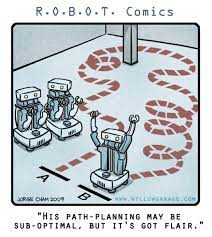
\includegraphics[width=0.5\textwidth]{Figures/path-planning-comic.jpeg}
    \decoRule
    \caption[]{Path Planning}
    \label{fig:Path Planning Comic}
\end{figure}


\subsection{Configuration Space}
An Industry 4.0 environment has broadly 2 types of objects, \textbf{robots} and \textbf{obstacles}. They are considered to be the part of the world.
Robot's motion for path planning that a robot could execute as a rigid body in it's degree of freedom while maintaining robot's constraints of movement. The constraints are the size of robot's base and the degree to which it can move.
The 'space' for the robot to move is possible coordinate motion space that can be applied for the robot to move in the environment without hitting an obstacle or obstructing the path of another robot.
We can use similar motion planning algorithms to different problems and robots which have other geometry and motion controls. Robot's configuration can be described by a vector containing joint coordiantes of the robot. These coordinates are either an angle or a length for rotational and sliding joint respectively.
Robot's Motion space is the environment space deducting the obstacle's space. 

\subsubsection{Minkowski Sum}
Minkowski Sum is used to calculate the vector configuration space of the robot as a whole. The sum of two sets of position vectors \textbf{A} and \textbf{B} are calculated by adding a those vectors with one another, forming the set
$A + B$ = $a + b$ $|$  $a \in A$ and $b \in B$
To compute free space and an obstacle space for the robot, we need the vecotrs for the static obstacle as well as the robot in relation to a specific reference point. So, in case the robot collide, we add those two positional vectors, the result provides the value of obstacle space.

\subsubsection{Path Planning Problem}
The objective of a path planning problem is to succesfully predict the next states of the robot which the robot would follow. A trajectory is defined as the path that the robot takes, the trajectory is/can be different from the planned predicted path because of drift and size of the robot matter while cutting sharp corners in the path.
Thus, in an Industry 4.0 environment a workspace, an obstacle region and a configuration space are defined. Suppose that we wish to go from Point A to Point B following the trajectory. The trajectory is calculated by a function where the initial and the final positions are both in the configuration space and the robot moves till the final destination coordiante is reached.
The path planning is done by ROS's architecture, specifically the navigation stack.

\begin{figure}[th]
\centering
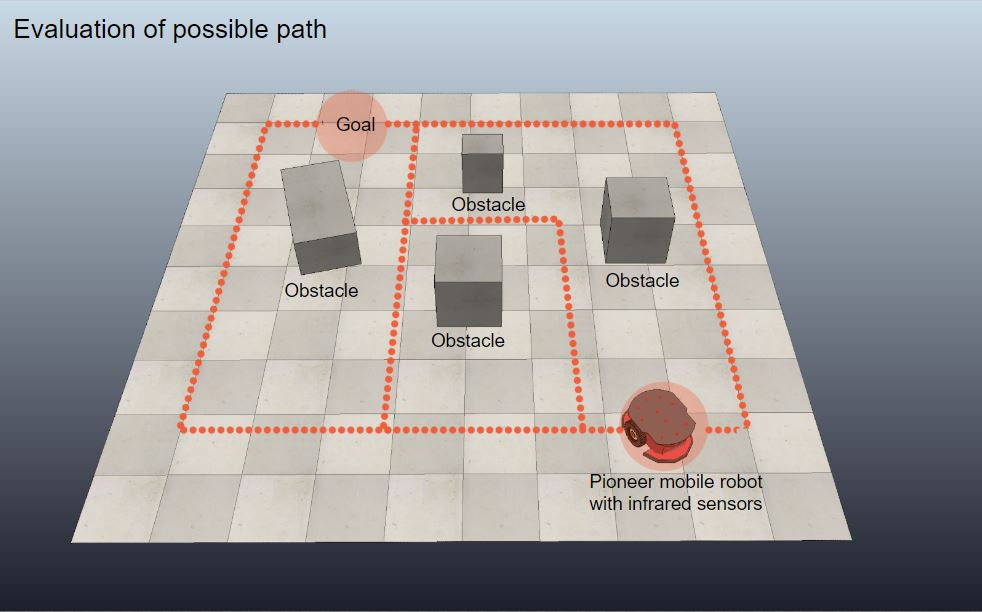
\includegraphics[width=0.8\textwidth]{Figures/path-planning-to-goal.jpg}
\decoRule
\caption[]{Evaluation of Possible Path to Goal.}
\label{fig:Path Planning}
\end{figure}

\begin{figure}[th]
    \centering
    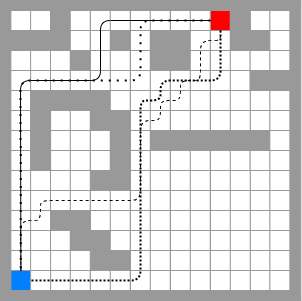
\includegraphics[width=0.6\textwidth]{Figures/14x14_grid_paths.png}
    \decoRule
    \caption{Possible ways of path planning.}
    \label{fig: Grid Paths}
\end{figure}

There are various different approaches to path planning which use the configuration space of the environment for succesful next state planning. The different solutions provide levels of completeness to the solution. In our context, the path planning provides a complete solution i.e \textit{If a solution exists, it will find one otherwise it will return a failure to form the path}. 
The work employs \textit{combinatorial method} to find the path to a goal state. 

\subsubsection{Combinatorial Method}
Combinatorial Method is employed to calculate a valid roadmap to access the connectivity to the final goal destination by maintaining the robot's constraints, with resoect to the obstacle space.
Combinatorial Method is executed in the following steps : 
\begin{itemize}
    \item Calculating the Configuration space, and dividing them into free/obstacle space. This is employed by using SLAM (Simultaneous Localization and Mapping) to develop a map for the configuration space.
    \item Generation of a roadmap in the free configuration space, i.e calculating the free space in which the robot can reach the goal, and once the robot reaches the destination the exploration stops.
    \item Computing the cost of the path from initial state to the final state, and choosing the path suited for implementation, for example, shortest path, optimal path or a path subjected to some constraints. It is totally user defined.
    \item The result is the final path in the free configuration zone.
\end{itemize}

\section{Digital Twins}
Digital Twin (DT) technology is now used and commercialized in various industries to optimize Industry 4.0 processes and environments. 
Digital Twin (DT) is used to model Industry 4.0 machine/process before it's inception in real-world using materials.
Making an artificial digital twin model before a physical twin is required. It helps researchers to model for training testing and preventing errors. 
Based on the artificial digital twin, the researchers can further study and train and improve upon the previous present model. DTs can be defined as (physical and/or virtual) machines
or computer-based models that are simulating, emulating 
mirroring, or ‘‘twinning’’ the life of a physical entity, which
may be an object, a process, a human, or a human-related feature. Each DT is linked to its physical twin through a unique
key \cite{8901113}. A digital twin can be visualized by a simulation, but a DT is not a simulation, instead it is much more than a simulation. Digital Twin is an exact replica of 
an real-world entity, which means that it is a living, intelligent model which can evolve if needed to. All the abilities and capabilities of the physical twin can be realized such as monitoring and control.
We could predict the future status of the digital twin, i.e we can predict future defects and failures. Digital Twin Techologies can enable continuous communication-collaboration-interaction with the 
physical twin simultaneously. Digital Twins are mostly a part of a Cyber-Physical System (CPS). To sum everything up, we can say that a Digital Twin is a technology which helps the researcher to 
utilize data fusion, Artificial Intelligence appliations with big data by using the IOT sensors without making the usual physical-twin.

In the context of our project, the cyber-physical system we have consists of a robot where we can employ different sensors to study it's behaviour in an Industry 4.0 environment. The robot is not supposed to have it's sensors do the computation.
The hypothesis is to make a digital twin, with a god's eye view which can see and then log the behaviour of the robot around the obstacles in the configuration space.

\section{Behavioural Learning}
Multi-Agent Systems are rapidly growing in usage in a variety of domains. Multi Agent Systems contain, as the name suggests, multiple entities. 
In environments, where multi-agent systems rapidly collaborate with one another, i.e a dynamic system. The agent needs to learn and improve on basic behaviour using data mining and reinforcement learning.
In the context of our project, the multi-agent system needs to prevent collision. Thus, we wish to learn the robot's behaviour around the obstacles in the particular space. For this, we note and log the position of the robot
at every step, and it's nearby obstacles to produce data for a reinforcement learning model.